\chapter[Introdução]{Introdução}
\label{cp:introducao}

\section{Apresentação do Tema}
\label{sec:apresentacao}

Um dos instrumentos mais fundamentais e que são cada vez mais crescentes na vida organizacional de uma empresa são as reuniões. Segundo \cite{allen2016}, já se gastam até 15\% do tempo coletivo da organização com reuniões.

Encontros institucionais que não são produtivas e sem sentido, é o que \cite{davidgrady} chama de "Síndrome de Aceitação Sem Sentido"(MAS). David define o MAS como "um reflexo involuntário em que uma pessoa aceita um convite de reunião sem sequer saber o porquê. Uma doença comum entre o escritório e trabalhadores em todo mundo". Atividades que deveriam ser simples e rápidas se tornam complicadas com várias reuniões para a execução completa delas. Reuniões não são nenhum ponto de prazer entre dentro de uma instituição, contudo se os próprios funcionários não conseguem ver o sentido da reunião e os tópicos abordados, mostra que a empresa como um todo está fadada ao fracasso.

Nesse viés, reuniões é um dos meios usados para programar uma atividade, reunir pessoas em busca de uma solução relacionada ao problema X. Composta por vários encontros sem tópicos e objetivos específicos, sem \textit{feedbacks} aos gerentes e sem atas sobre o que foi discutido, as reuniões infelizmente se tornam um problema para gerentes e seus funcionários para as instituições. Problemas como estes podem ser pela falta de investimento disponível para aplicação na área tecnológica ou até mesmo pela priorização de outras necessidades.

Este trabalho visa propor uma solução de \textit{software} para auxiliar a condução de reuniões, utilizando dos conhecimentos adquiridos no curso de \imprimircurso para o desenvolvimento de uma solução que se adeque às reais necessidades empregadas aos gerentes dos projetos organizacionais.

\section{Justificativa}
\label{sec:justificativa}

Tendo como premissas os problemas em reuniões apresentados no tópico anterior (\ref{sec:apresentacao}), uma das soluções para aumentar a produtividade em reuniões é através de um sistema \textit{web} que auxilie os gerentes e líderes de reuniões a gerenciar seus encontros de forma rápida, intuitiva e gratuita para que qualquer organização possa usar os recursos do \textit{software} com o objetivo de melhorar a organização de sua empresa.

O Sistema GRATA, vem oferecer a solução prática para a melhoria do controle das informações e qualidade dos serviços. Tendo como a principal funcionalidade o registro das Atas de reuniões de forma simples e intuitiva, tanto para quem gerencia como para quem participa. Além da automação dos processos essenciais da organização, o sistema fornece relatórios gerenciais e analíticos, que podem ser usados para identificação de pontos de melhoria ou até mesmo para dar visibilidade a questões específicas.

\section{Problema de Pesquisa}
\label{sec:problema_de_pesquisa}

O crescente problema com reuniões mal gerenciadas seja por gerentes não capacitados, ou por falta da especificação prévia dos tópicos a serem abordados, levam diretamente a reuniões mal sucessididas e com isso desperdício de tempo e dinheiro. Estima-se que empresas gastam em média US \$ 37 bilhões anualmente em reuniões \cite{baer}. O custo real desses encontros impulsionou a \cite{harvard} a criar uma calculadora que ajuda gerentes a calcularem o verdadeiro custo de um encontro.

Nessa viés e utilizando a justificativa desenvolvida no tópico \ref{sec:justificativa}, é possível se ter o problema de pesquisa. A problemática a ser resolvida neste projeto é: \textit{Como desenvolver um sistema para auxiliar a condução de reuniões em organizações?}

\subsection{Metodologia}
\label{sec:metodologia_introducao}

A metodologia abordada neste trabalho teve sua escolha baseada após a realização de pesquisas comparativas entre metodologias tradicionais como o \cite{pmbok} e a metodologia ágil de \textit{software}.

Por conta de um conhecimentos maior sobre a metodologia e com entregas frequentes em menos tempo, a metodologia escolhida para este projeto no desenvolvimento do sistema foi a metodologia ágil, juntamente com algumas práticas do \textit{Scrum} e baseado nos valores do \textit{Lean Software Development}.

\subsection{Requisitos}
\label{sec:requisitos_introducao}

Requisito não é um termo usado apenas pela \imprimircurso. Há casos em que requisitos são apenas uma declaração abstrata em alto nível de um serviço ou restrição que um sistema deve oferecer.

\cite{sommerville} os define como: "Os requisitos de um sistema são as descrições do que o sistema deve fazer, os serviços que oferece e as restrições a seu funcionamento. Esses requisitos refletem as necessidades dos clientes para um sistema que serve a uma finalidade determinada, como controlar um dispositivo, colocar um pedido ou encontrar informações."

Requisitos podem ser definidos em duas categorias: Requisitos Funcionais e Requisitos Não-Funcionais, ambos serão definidos a seguir.

\subsubsection{Requisitos Funcionais}
\label{sec:requisitos_funcionais_introducao}

Os requisitos funcionais descreve o que o sistema deve de fato ser. Requisitos funcionais podem ser tão específicos quanto necessário,por exemplo, podem ter sistemas com requisitos funcionais gerais e outros que além de refletir os sistemas, também abrangem as formas de trabalho de uma organização. Requisitos funcionais de um sistema deve ser completo, isso quer dizer que todos os serviços requisitados pelo usuário devem ser definidos.

\subsubsection{Requisitos Não-Funcionais}
\label{sec:requisitos_nao_funcionais_introducao}

Requisitos não-funcionais são requisitos que são relacionados as propriedades do sistema como confiabilidade, tempo de espera, desempenho, segurança e até restrições do sistema. Requisitos não-funcionais podem possui tanta relevância quanto os requisitos funcionais, pois em uma reunião de levantamento de requisitos, o cliente sonha o mundo e não está atento se os recursos os próprios recursos e os recursos da emprega conseguem atender ao requisito. Um requisito não-funcional não atendido pode inclusive inutilizar um projeto. Exemplo disso é caso um sistema de uma aeronave não consiga atingir a confiabilidade necessária, não será dado o certificado de segurança para operar, sendo assim a aeronave não poderá voar.

\subsection{Processo de Desenvolvimento de Software}

Segundo \cite{sommerville}, esse processo pode ser definido como "Um processo de \textit{software} é um conjunto de atividades relacionadas que levam à produção de um produto de \textit{software}."

Neste trabalho, foram definidas as principais atividades a serem realizadas para alcançar o objetivo final de ter um sistema gratuito que auxilie os gerentes a otimizar suas reuniões por meio computacional:

\begin{itemize}
    \item Especificação do \textit{software}: funcionalidades e restrições do \textit{software};
    \item Projeto e implementação do \textit{software}: as especificações que o \textit{software} deve atender;
    \item Validação de \textit{software}: para que atenda as expectativas do cliente, o \textit{software} deve ser validado pelo mesmo;
    \item Evolução do \textit{software}: o \textit{software} deve ser capaz de ser extensível a mudanças, tendo assim seu código aberto.
\end{itemize}

É nessa fase que são definidas a arquitetura e a linguagem de \textit{software}.

\subsection{Linguagem de Software}

Linguagem de programação são instruções passadas de maneira que o computador entenda e apresente um retorno. Existem diversas linguagens de programação, desde a mais baixo a alto nível.

Linguagens de \textit{software}, como também podem ser chamadas, são divididas em duas frentes: \textit{front-end} e \textit{back-end}. Ambas serão explicadas nos tópicos a seguir.

\subsubsection{Front-end}

A programação de um \textit{software} pelo ponto de vista do \textit{front-end} é a visão final do usuário com o sistema. \textit{Front-end} é a responsável pela interação do usuário com o sistema e essa interação é dada a partir de telas/páginas. Existem diversos tipos de \textit{frameworks} que auxiliam os desenvolvedores a trabalhar com essa frente, como:

\begin{itemize}
    \item \textit{Bootstrap
    \item Materialize
    \item React
    \item Angular 4}
\end{itemize}

A linguagem \textit{front-end} escolhida para este projeto, foi o \textit{React}, pois além de facilitar o desenvolvimento e interação com usuário final, é uma das mais utilizadas ao redor do mundo, então é facilita uma manutenção futura do \textit{software}.

\subsubsection{Back-end}

A programação \textit{back-end} possui as responsabilidades de receber os dados pelo \textit{React}, que é o \textit{front-end} deste projeto, possui o dever de tratar os dados, valida-los e fomentá-los a visão do usuário.

Existem diversas linguagens \textit{back-end} que auxiliam os desenvolvedores a trabalhar em uma linguagem que o computador entende, como:

\begin{itemize}
    \item \textit{Python Django-Rest
    \item Java
    \item Ruby on Rails
    \item PHP}
\end{itemize}

A linguagem \textit{back-end} escolhida para este projeto, foi a \textit{Python Django-Rest}, pois tem uma ótima conexão com a linguagem \textit{front-end}, e por ser muito utilizada, possibilita assim uma manutenção futura.

\subsection{Arquitetura de Software}

A arquitetura de \textit{software} é como o sistema deve ser organizado com a estrutura geral do projeto. A arquitetura possui um valor alto dentro da construção de um \textit{software}, pois nela se tem o elo entre o projeto e a engenharia de requisitos. Possui o dever identificar os principais componentes estruturais no sistema e o relacionamento entre eles. Neste projeto a arquitetura adotada é uma adaptação ao padrão arquitetural MVC \textit{(model-view-controller)}.

\subsubsection{Model-View-Controller}
\label{sec:mvc}

O padrão arquitetural MVC é responsável de responsabilidades em camadas. A primeira é \textit{Model}(modelo), que é responsável pela manipulação de dados, ou seja, leitura, escrita de dados e também suas validações é de responsabilidade da Model. A segunda camada é a \textit{View}(visão), que possui a responsabilidade de interação com o usuário. Por último se tem a \textit{Controller}(controladora), responsável por receber as aquisições do usuário. A controller também tem o dever de disponibilizar os dados para a \textit{view} e assim ocorrer a interação com o usuário.

\subsubsection{Arquitetura do Projeto}

Neste projeto é feita uma adaptação ao padrão MVC, por conta da escolha da linguagem \textit{front-end}. O \textit{React} possui um padrão arquitetural diferente, chamado de arquitetura de componentes/microserviços. Esse padrão possui semelhanças ao MVC, e o que será utilizado dele será a parte da \textit{View}. Enquanto a linguagem \textit{back-end} é responsável por trabalhar os dados provindos do \textit{front-end} e oferecer um retorno a ele. 

A seguir será mostrado como funciona separadamente o \textit{React},relacionado ao \textit{front-end} que engloba a \textit{View}, enquanto o \textit{Python Django-Rest} é responsável pelo \textit{back-end} e que engloba a \textit{Model} e a \textit{Controller}:

\begin{figure}[H]
	\centering
	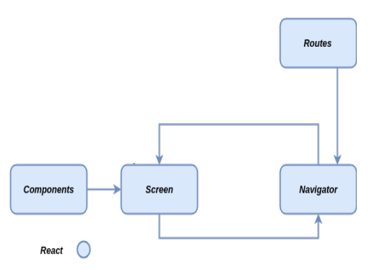
\includegraphics[width=1.0\textwidth]{figuras/diagrama_react.png}
	\caption{Diagrama React/Microsserviços}
	\label{img:diagrama_react}
\end{figure}

\begin{figure}[H]
	\centering
	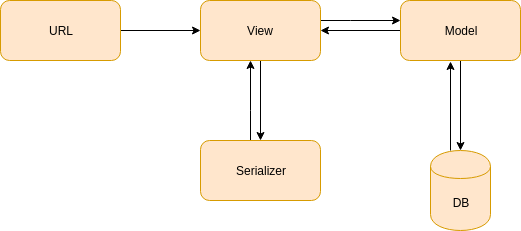
\includegraphics[width=1.0\textwidth]{figuras/django_rest.png}
	\caption{Diagrama Django REST Framework}
	\label{img:diagrama_rest}
\end{figure}



\section{Objetivos}
\label{sec:objetivos}

\subsection{Objetivos Gerais}
\label{sec:objetivos_gerais}

O objetivo do projeto é propor novos processos de reuniões e gerenciamento dos documentos gerados no ciclo de desenvolvimento dos projetos, contando com o suporte de um software gratuito e de código aberto para automatizar alguns dos trabalhos manuais, tornando os processos mais ágeis e com armazenamentos seguros.

\subsection{Objetivos Específicos}
\label{sec:objetivos_especificos}

\begin{itemize}
    \item Criar um \textit{software} que auxilie gerentes e líderes a terem reuniões mais objetivas;
    \item implementar mecanismos que permita o controle gerencial das reuniões;
    \item permitir o controle de todas as informações provindas das reuniões.
\end{itemize}
